\tikzset{every picture/.style={line width=0.75pt}} %set default line width to 0.75pt        

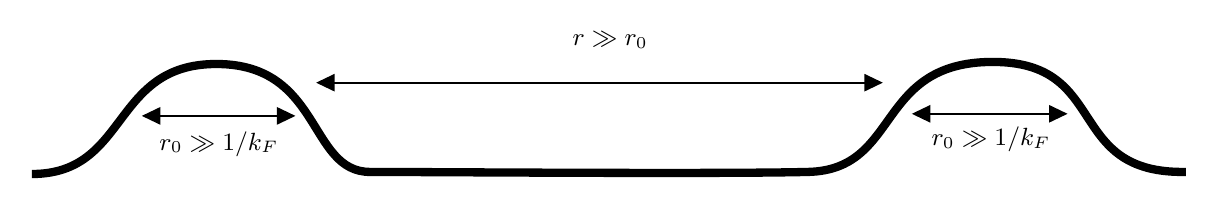
\begin{tikzpicture}[x=0.75pt,y=0.75pt,yscale=-1,xscale=1]
%uncomment if require: \path (0,300); %set diagram left start at 0, and has height of 300

%Curve Lines [id:da6730178697421663] 
\draw [line width=3]    (33,125) .. controls (80,125) and (71.06,71.93) .. (122,72) .. controls (172.94,72.07) and (166,124) .. (196,124) .. controls (226,124) and (361.98,125.09) .. (407,124) .. controls (452.02,122.91) and (439,71) .. (496,71) .. controls (553,71) and (530,125) .. (589,124) ;
%Straight Lines [id:da11185223986826509] 
\draw    (89,97) -- (157,97) ;
\draw [shift={(160,97)}, rotate = 180] [fill={rgb, 255:red, 0; green, 0; blue, 0 }  ][line width=0.08]  [draw opacity=0] (8.93,-4.29) -- (0,0) -- (8.93,4.29) -- cycle    ;
\draw [shift={(86,97)}, rotate = 0] [fill={rgb, 255:red, 0; green, 0; blue, 0 }  ][line width=0.08]  [draw opacity=0] (8.93,-4.29) -- (0,0) -- (8.93,4.29) -- cycle    ;
%Straight Lines [id:da08396554987934568] 
\draw    (460,96) -- (529,96) ;
\draw [shift={(532,96)}, rotate = 180] [fill={rgb, 255:red, 0; green, 0; blue, 0 }  ][line width=0.08]  [draw opacity=0] (8.93,-4.29) -- (0,0) -- (8.93,4.29) -- cycle    ;
\draw [shift={(457,96)}, rotate = 0] [fill={rgb, 255:red, 0; green, 0; blue, 0 }  ][line width=0.08]  [draw opacity=0] (8.93,-4.29) -- (0,0) -- (8.93,4.29) -- cycle    ;
%Straight Lines [id:da1160594665438861] 
\draw    (173,81) -- (440,81) ;
\draw [shift={(443,81)}, rotate = 180] [fill={rgb, 255:red, 0; green, 0; blue, 0 }  ][line width=0.08]  [draw opacity=0] (8.93,-4.29) -- (0,0) -- (8.93,4.29) -- cycle    ;
\draw [shift={(170,81)}, rotate = 0] [fill={rgb, 255:red, 0; green, 0; blue, 0 }  ][line width=0.08]  [draw opacity=0] (8.93,-4.29) -- (0,0) -- (8.93,4.29) -- cycle    ;

% Text Node
\draw (93,103) node [anchor=north west][inner sep=0.75pt]  [font=\small] [align=left] {$\displaystyle r_{0} \gg 1/k_{F}$};
% Text Node
\draw (292,55) node [anchor=north west][inner sep=0.75pt]  [font=\small] [align=left] {$\displaystyle r\gg r_{0}$};
% Text Node
\draw (465,101) node [anchor=north west][inner sep=0.75pt]  [font=\small] [align=left] {$\displaystyle r_{0} \gg 1/k_{F}$};


\end{tikzpicture}


